\providecommand{\main}{../..}
\documentclass[\main/notes.tex]{subfiles}

\begin{document}
	\setcounter{chapter}{7}
	\chapter{Management Information and Decision Support Systems}
	\chaptermark{MIS and DSS}
		\section{Decision-Making and Problem-Solving}
			\begin{definition}{Decision-Making Phase}
				The first part of problem-solving, including three stages: intelligence, design, and choice.
			\end{definition}
			\begin{definition}{Problem-Solving}
				A process that goes beyond decision-making to include the implementation and monitoring stages.
			\end{definition}
			\begin{sidenote}{Decision-Making and Problem-Solving}
				\begin{minipage}{0.39\textwidth}
					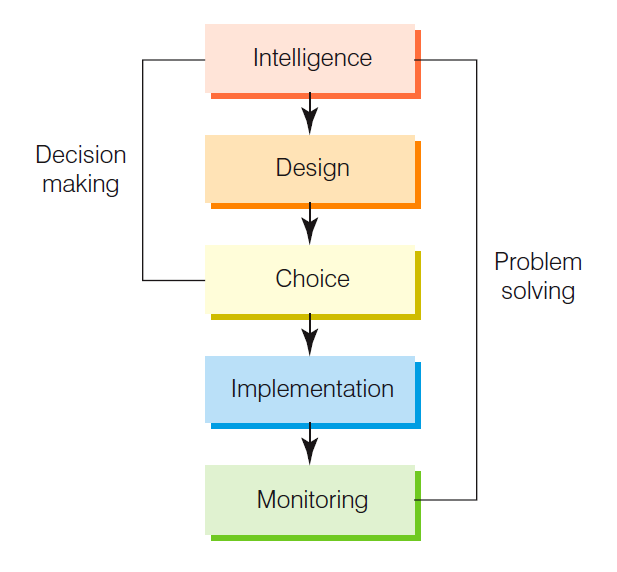
\includegraphics[width=0.9\linewidth]{chapter08/decision_making.png}
				\end{minipage}
				\begin{minipage}{0.6\textwidth}
					\begin{description}[]
						\item[Intelligence Stage] The first stage of decision-making, in which problems or opportunities are identified and defined.
						\item[Design Stage] The second stage of decision-making, in which alternative solutions to the problem are defined.
						\item[Choice Stage] The third stage of decision-making, which requires selecting a course of action.
						\item[Implementation Stage] A stage of problem-solving, in which a solution is put into effect.
						\item[Monitoring Stage] The final stage of the problem-solving process, in which decision-makers evaluate the implementation.
					\end{description}
				\end{minipage}
			\end{sidenote}
			\subsection{Programmed vs Non-Programmed Decisions}
				\begin{definition}{Programmed Decision}
					A decision made using a rule, procedure, or quantitative method.

					East to computerise using traditional information systems. They are structured, and deal with routine, well-defined decisions.
				\end{definition}
				\begin{definition}{Non-programmed Decision}
					A decision that deals with unusual or exceptional situations that can be difficult to quantify.
				\end{definition}
			\subsection{Optimisation, Satisficing, and Heuristic Approaches}
				\begin{definition}{Optimisation Model}
					A model that finds the best solution. These models use problem constraints.
				\end{definition}
				\begin{definition}{Satisficing Model}
					A model that will find a good, but not necessarily the best, problem solution.

					Usually used because modelling the problem properly to get an optimal decision would be too difficult, complex, or costly.

					Satisficing does not look at all possible solutions, but only those likely to give good results.
				\end{definition}
				\begin{definition}{Heuristics}
					Often referred to as \concept{rules of thumb}. Commonly accepted guidelines of procedures that usually find a good solution.
				\end{definition}
			\subsection{Sense and Respond}
				\begin{definition}{Sense and Respond (SaR)}
					Determining problems or opportunities (\concept{sense}), and developing systems to solve the problems or take advantage of the opportunities (\concept{respond}).

					Requires nimble organisations that replace traditional lines of authority with those that are flexible and dynamic.
				\end{definition}
			\subsection{Big Data}
				\begin{definition}{Big Data}
					Where the data that a company collects is so huge that it is difficult to process using traditional database technology.
				\end{definition}

		\pagebreak
		\section{An Overview of Management Information Systems}
			\begin{definition}{Management Information System (MIS)}
				An integrated collection of people, procedures, databases, hardware, and software, that provides managers and decision-makers with information to help achieve organisational goals.

				The primary purpose of an MIS is to help an organisation achieve its goals, by providing managers with insight into the regular operations of the organisation, so that they can control, organise, and plan more effectively.
			\end{definition}
			\subsection{Inputs to a Management Information System}
				Data enters an MIS from both internal and external sources.

				The most significant internal data sources are the organisation's various ERP and TPS systems.

				External sources of data can include customers, suppliers, competitors and stockholders, as well as other sources, such as the Internet.
			\subsection{Outputs of a Management Information System}
				The output is typically a collection of reports that are distributed to managers. These can include tabulations, summaries, charts, and graphs.
				\begin{definition}{Scheduled Reports}
					Reports that are produced periodically, or on a schedule, such as daily, weekly, or monthly.
				\end{definition}
				\begin{definition}{Key-Indicator Reports}
					Reports that summarise the previous day's critical activities. Typically, available at the beginning of each workday.

					Used to take quick, corrective action on significant aspects of the business.
				\end{definition}
				\begin{definition}{Demand Reports}
					Reports that are developed to give certain information at someone's request.
				\end{definition}
				\begin{definition}{Exception Reports}
					Reports that are automatically produced when a situation is unusual, or requires managerial action.
				\end{definition}
				\begin{definition}{Drill-down Reports}
					Reports that provide increasingly detailed data about a situation.

					Analyst can see data at a high level first, then at a more detailed level, then at a very detailed level.
				\end{definition}
				\begin{sidenote}{Developing Effective Reports}
					\begin{multicols}{2}
						\begin{itemize}[nosep]
							\item Tailor each report to user needs
							\item Spend time and effort producing only reports that are useful
							\item Pay attention to report content and layout
							\item Use management-by-exception reporting
							\item Set parameters carefully
							\item Produce all reports in a timely fashion
							\item Periodically review reports
						\end{itemize}
					\end{multicols}
				\end{sidenote}
			\subsection{Characteristics of a Management Information System}
				\begin{sidenote}{Functions of an MIS}
					\begin{multicols}{2}
						\begin{itemize}[nosep]
							\item Provide reports with fixed and standard formats
							\item Produce hard-copy and soft-copy reports
							\item Use internal data stored in the computer system
							\item Allow users to develop their own custom reports
							\item Require users to submit formal requests for reports to systems personnel
						\end{itemize}
					\end{multicols}
				\end{sidenote}

		\section{Functional Manufacturing Information Systems}
			\subsection{Financial Management Information Systems}
				\begin{definition}{Financial Management Information System}
					A management information system that provides financial information, not only for executives, but also for a broader set of people who need top make better decisions on a daily basis.
				\end{definition}
				\begin{sidenote}{Functions of a Financial MIS}
						\begin{itemize}[nosep]
							\item Integrate financial and operational information from multiple sources, including the Internet, into a single system.
							\item Provide easy access to data for both financial and non-financial users, often through the use of a corporate intranet.
							\item Make financial data immediately available to shorten analysis turnaround time
							\item Enable analysis of financial data along multiple dimensions
							\item Analyse historical and current financial activity
							\item Monitor and control the use of funds over time
						\end{itemize}
					Used to compute revenues, costs, profits, \concept{auditing}, as well as to manage funds.
					\begin{definition}{Auditing}
						Analysing the financial condition of an organisation, and determining whether financial statements and reports produced by the financial MIS are accurate.
					\end{definition}
				\end{sidenote}
			\subsection{Manufacturing Management Information Systems}
				\begin{definition}{Manufacturing Information System}
					A management information system that allows greater control over the manufacturing process.

					The manufacturing MIS subsystems and outputs monitor and control the flow of materials, products, and services throughout the organisation.
				\end{definition}
				\begin{sidenote}{Common Information Subsystems and Outputs in Manufacturing}
					\begin{description}
						\item[Design and engineering] Manufacturing companies often use \concept{computer-aided design (CAD)} with new or existing products.
						\item[Master production scheduling and inventory control] Provide detailed plans for both short-term and long-range scheduling of manufacturing facilities.
							\begin{description}[nosep]
								\item[Economic Order Quantity (EOQ)] The quantity that should be reordered to minimise total inventory costs.
								\item[Reorder Point (ROP)] A critical inventory quantity level.
								\item[Material Requirements Planning (MRP)] A set of inventory-controlled techniques that help coordinate thousands of inventory items when the demand for one item is dependent on the demand for another.
								\item[Just-in-time (JIT) Inventory] A philosophy of inventory management in which inventory and materials are delivered just before they are used in manufacturing a product.
							\end{description}
						\item[Process Control] Technologies used to control and streamline the manufacturing process.
							\begin{description}[nosep]
								\item[Computer-Aided Manufacturing (CAM)] A system that directly controls manufacturing equipment.
								\item[Computer-Integrated Manufacturing] Using computers to link the components of the production process into an effective system.
								\item[Flexible Manufacturing System (FMS)] An approach allowing manufacturing facilities to rapidly and efficiently change from making one product to making another.
							\end{description}
						\item[Quality Control] A process that ensures that the finished product meets the customer's needs.
					\end{description}
				\end{sidenote}
			\subsection{Marketing Management Information Systems}
				\begin{definition}{Marketing Management Information System}
					An information system that supports managerial activities in product development, distribution, pricing decisions, promotional effectiveness, and sales forecasting.
					\begin{description}
						\item[Customer Relationship Management (CRM)] Help a company manage all aspects of customer encounters. 
					\end{description}
				\end{definition}
				\pagebreak
				\begin{sidenote}{Subsystems of Marketing MIS}
					\begin{description}
						\item[Marketing Research] Conduct a formal study of the market and customer preferences.
						\item[Product Development] The conversion of raw materials into finished goods and services, focuses primarily on the physical attributes of the product.
						\item[Promotion and Advertising]
						\item[Product Pricing] Retail price, wholesale price, and price discounts must be set.
						\item[Sales Analysis] Identify products, sales personnel, and customers that contribute to profits, and those that do not.
							\begin{description}[nosep]
								\item[Sales-by-product report] Lists all major products and their sales for a period of time.
								\item[Sales-by-salesperson] Lists total sales for each salesperson. Can also be subdivided by product.
								\item[Sales-by-customer] Used to identify high- and low-volume customers.
							\end{description}
					\end{description}
				\end{sidenote}
			\subsection{Human Resource Management Information Systems}
				\begin{definition}{Human Resource Management Information System (HRMIS)}
					Also called a \concept{personnel MIS}. An information system that is concerned with activities related to employees and potential employees of an organisation.
				\end{definition}
				\begin{sidenote}{Subsystems of HRMIS}
					\begin{description}
						\item[Human Resource Planning] Put the right number and kinds of employees in the right jobs when they are needed.
						\item[Personnel Selection and Recruiting]
						\item[Training and Skills Inventory]
						\item[Scheduling and Job Placement]
						\item[Wage and Salary Administration]  
					\end{description}
				\end{sidenote}
			\subsection{Geographic Information Systems}
				\begin{definition}{Geographic Information System (GIS)}
					A computer system capable of assembling, storing, manipulating and displaying \concept{geographic information} (data that is identified according to its location).
					\begin{description}
						\item[Geographic Information] Data identified according to its location.
					\end{description}
				\end{definition}

		\section{Decision Support Systems}
			\begin{definition}{Decision Support System (DSS)}
				An organised collection of people, procedures, software, databases and devices, used to help make decisions that solve problems.

				The focus of a DSS is on decision-making effectiveness when faced with unstructured or semi-structured business problems.
			\end{definition}
			\begin{sidenote}{Characteristics of a Decision Support System}
				\begin{itemize}[nosep]
					\item Provide rapid access to information.
					\item Handle large amounts of data from different sources.
					\item Provide report and presentation flexibility
					\item Offer both textual and graphical orientation
					\item Support drill-down analysis
					\item Perform complex, sophisticated analysis and comparisons using advanced software packages.
					\item Support optimisation, satisficing, and heuristic approaches. Gives the decision-maker a great deal of flexibility.
						\begin{description}
							\item[What-If Analysis] The process of making hypothetical changes to problem data, and observing the impact on the results.
						\end{description}
					\item Perform goal-seeking analysis.
						\begin{description}
							\item[Goal-seeking Analysis] The process of determining the problem data required for a given result.
						\end{description}
					\item Perform simulation.
						\begin{description}
							\item[Simulation] The ability of the DSS to duplicate the features of a real system.
						\end{description}
				\end{itemize}
			\end{sidenote}
			\begin{sidenote}{Capabilities of a Decision Support System}
				\begin{itemize}[nosep]
					\item Support for problem-solving phases.
					\item Support for different decision-frequencies. Decisions can range on a continuum from one-of-a-kind to repetitive decisions.
						\begin{description}[nosep]
							\item[Ad Hoc DSS] A DSS concerned with situations or decisions that come up only  few times during the life of the organisation.
							\item[Institutional DSS] A DSS that handles situations or decisions that occur more that once, usually several times per year or more. An institutional DSS is used repeatedly, and refined over the years.
						\end{description}
					\item Support for different problem structures.
						\begin{description}[nosep]
							\item[Highly Structured Problems] Problems that are straightforward, and require known facts and relationships.
							\item[Semi-Structured or Unstructured Problems] Complex problems where the relationships between the pieces of data are not always clear. The data might be in a variety of formats, and the data is often difficult to manipulate or obtain.
						\end{description}
					\item Support for various decision-making levels.
				\end{itemize}
			\end{sidenote}
			\subsection{Comparison of a DSS and an MSS}
				\begin{center}
					\begin{tblr}{colspec={>{\raggedright}X[2]>{\raggedright}X[3]>{\raggedright}X[3]}, row{even}={table even}, row{1}={font=\bfseries}, column{1}={font=\bfseries}}
						\toprule
						Factor & DSS & MIS\\
						\midrule
						Problem Type & Unstructured Problems & Structured Problems\\
						Users & Individuals, small groups, and the entire organisation & Primarily the organisation\\
						Support & All aspects and phases of decision-making. Does \emph{not} replace the decision-maker & Some make automatic decisions and replace the decision-maker\\
						Emphasis Approach & Emphasises decisions and decision-making styles. A direct support system & Emphasises information only. An indirect support system\\
						Speed & A DSS is flexible and can be implemented by users, so it usually takes less time to develop, and is better able to respond to user requests & Longer response time.\\
						Output & Usually screen-oriented, with the ability to generate reports on a printer & Oriented towards printed reports and documents\\
						Development & Users are usually more directly involved. Usually means better systems that provide superior support. & Frequently several years old, and was developed for people who are no longer doing the work supported by the MIS.\\
						\bottomrule
					\end{tblr}
				\end{center}
			\subsection{Components of a Decision Support System}
				At the core of a DSS are a database and a model base. In addition, a typical DSS contains a user interface, also called a \concept{dialogue manager}.
				\begin{definition}{Dialogue Manager}
					A user interface that allows decision makers to easily access and manipulate the DSS, and to use common business terms and phrases.
				\end{definition}
				\subsubsection{The Database}
					\begin{definition}{Database Management System}
						Allows managers and decision makers to perform qualitative analysis on the company's vast stores of data in databases and data warehouses.
					\end{definition}
				\subsubsection{The Model Base}
					\begin{definition}{Model Base}
						Part of a DSS that provides decision makers with access to a variety of models, and assists them in decision-making.
					\end{definition}
					\begin{definition}{Model Management Software}
						Software that coordinates the use of models in a DSS.
					\end{definition}

		\section{Group Support Systems}
			\begin{definition}{Group Support System (GSS)}
				Also called a \concept{group decision support system}. A software application that consists of most elements in a DSS, plus software to provide effective support in group decision-making.

				Any technology that allows groups of people to interact could be labelled a GSS.
			\end{definition}
			\begin{sidenote}{Characteristics of a GSS that Enhance Decision Making}
				\begin{itemize}[nosep]
					\item Design for groups
					\item Ease of use
					\item Flexibility
					\item Decision-Making Support
						\begin{description}[nosep]
							\item[Brainstorming] A decision-making approach that often consists of members offering ideas `off the top of their heads'.
							\item[Group Consensus Approach] A decision-making approach that forces members in the group to reach a unanimous decision.
							\item[Nominal Group Technique] A decision-making approach that encourages feedback from individual group members, and the final decision is made by voting, similar to the way public officials are elected.
						\end{description}
					\item Anonymous input
					\item Reduction of negative group behaviour
						\begin{description}
							\item[Groupthink] Members of a group assume they have made the right decision, without examining alternatives.
						\end{description}
					\item Parallel communication
					\item Automated record-keeping
				\end{itemize}
			\end{sidenote}

		\pagebreak
		\section{Executive Support Systems}
			\begin{definition}{Executive Support System}
				A specialised DSS that includes all hardware, software, data, procedures and people used to assist senior-level executives within the organisation. Also called an \concept{executive information system (EIS)}.

				DSS's provide a variety of modelling and analysis tools to enable users to thoroughly analyse problems, whereas ESS's present structured information about aspects of the organisation that executives consider important.
			\end{definition}
			\begin{sidenote}{Characteristics of an ESS}
				\begin{itemize}[nosep]
					\item Are tailored to individual executives
					\item Are easy to use
					\item Have drill-down abilities
					\item Support the need for external data
					\item Can help with situations that have a high degree of uncertainty
					\item Have a future orientation
					\item Are linked with value-added business processes
				\end{itemize}
			\end{sidenote}
			\begin{sidenote}{Capabilities of Executive Support Systems}
				\begin{itemize}[nosep]
					\item Support for defining an overall vision
					\item Support for strategic planning
						\begin{description}[nosep]
							\item[Strategic Planning] Determine the long-term objectives of an organisation, by analysing its strengths and weaknesses, and predicting future trends and projecting the development of new product lines.
						\end{description}
					\item Support for strategic organising and staffing
					\item Support for strategic control
						\begin{description}
							\item[Strategic Control] Monitoring and managing the overall operation of the organisation
						\end{description}
					\item Support for crisis management
				\end{itemize}
			\end{sidenote}

		\pagebreak
		\section{Exercises}
			\begin{exercise}{Self-Assessment}
				\begin{enumerate}[nosep]
					\item The first stage in decision-making is the \concept{intelligence} stage.
					\item A programmed decision can be made by a computer following a \concept{rule}.
					\item A model that produces a good enough decision is called \concept{satisficing}.
					\item Most of the data for an MIS comes from a \concept{TPS}.
					\item A regular, periodic report is called \concept{scheduled}.
					\item An MIS that supports promotional effectiveness is a \concept{Marketing} MIS.
					\item GIS stands for \concept{Geographic Information System}.
					\item Making hypothetical changes to data and observing the results is \concept{what-if analysis}.
					\item A GSS supports decision-making by a \concept{group}.
					\item A decision-making approach that encourages ideas `off the top' of participants' heads is \concept{brainstorming}.
				\end{enumerate}
			\end{exercise}

	\vbox{\rulechapterend}
\end{document}